%%%%%%%%%%%%%%%%%%%%%%%%%%%%%%%%%%%%%%%%%%%%%%%%%%%%%%%%%%%%%%%%%%%%%
%%%%%%%%%%%%%%%%%%%%%%%%%%%%%%%%%%%%%%%%%%%%%%%%%%%%%%%%%%%%%%%%%%%%%
%%%%%%%%%%%%%%%%%%%%%%%%%%%%%%%%%%%%%%%%%%%%%%%%%%%%%%%%%%%%%%%%%%%%%
%%%%%%%%%%%%%%%%%%%%%%%%%%%%%%%%%%%%%%%%%%%%%%%%%%%%%%%%%%%%%%%%%%%%%
\chapter{Linux-only AccessGrid}\label{kap:LinuxNode}
%%%%%%%%%%%%%%%%%%%%%%%%%%%%%%%%%%%%%%%%%%%%%%%%%%%%%%%%%%%%%%%%%%%%%
%%%%%%%%%%%%%%%%%%%%%%%%%%%%%%%%%%%%%%%%%%%%%%%%%%%%%%%%%%%%%%%%%%%%%
%%%%%%%%%%%%%%%%%%%%%%%%%%%%%%%%%%%%%%%%%%%%%%%%%%%%%%%%%%%%%%%%%%%%%
%%%%%%%%%%%%%%%%%%%%%%%%%%%%%%%%%%%%%%%%%%%%%%%%%%%%%%%%%%%%%%%%%%%%%

V~tejto kapitole popíšeme výstavbu uzla založeného na voľne dostupných komponentoch. Ako základ architektúry použijeme existujúci AG uzol v~organizácii Ciant. Naším príspevkom pre AG komunitu je niekoľko aplikácií voľne dostupných na wiki-stránkach projektu \cite{CIANT-AGnodeWiki}. V súvislosti so zdieľanými aplikáciami spomenieme hlavne SharedMPlayer.

\paragraph*{Fundamental rules:}
\begin{paklist}
\item Znížiť množstvo potrebného hardwaru na minimum.
\item Sprístupniť pripojenie uzlom za firewallom a NAT.
\item Využiť operačný systém Linux a voľne dostupné komponenty.
\end{paklist}

%%%%%%%%%%%%%%%%%%%%%%%%%%%%%%%%%%%%%%%%%%%%%%%%%%%%%%%%%%%%%%%%%%%%%
%%%%%%%%%%%%%%%%%%%%%%%%%%%%%%%%%%%%%%%%%%%%%%%%%%%%%%%%%%%%%%%%%%%%%
\section{Emplacement}
%%%%%%%%%%%%%%%%%%%%%%%%%%%%%%%%%%%%%%%%%%%%%%%%%%%%%%%%%%%%%%%%%%%%%
%%%%%%%%%%%%%%%%%%%%%%%%%%%%%%%%%%%%%%%%%%%%%%%%%%%%%%%%%%%%%%%%%%%%%

Podľa E. Hladkej a P. Holuba \cite{ArticleUVTMU-KomunikaceAGPoint}, je potrebné pred implementáciou videokonferenčného uzla zvážiť jeho priestorovú náročnosť. Uvádza sa \cite{AG-MinimumReqirements}, že je potrebné vyhradiť miesto aspoň pre troch účastníkov, počítače a projekčnú techniku. Inak nemá zmysel uvažovať o~jeho vytvorení. Musíme však rozlišovať medzi plnohodnotným videokonferenčným uzlom, mobilným videokonferenčným uzlom \cite{ArticleUVTMU-MobilniUzelAG} a tzv. personal interface to grid (PIG), ktorý má zabezpečiť pripojenie pre jednotlivcov bez použitia drahej projekčnej techniky. Rozdiely sú hlavne v~množstve potrebného hardware. Zatiaľ čo pri výstavbe plnohodnotného alebo mobilného uzla uvažujeme o~použití niekoľkých projektorov, v~prípade AG PIG vystačí účastník aj s~jedným prenosným počítačom dokonca bez vlastnej kamery a mikrofónu. Má teda na výber, či chce pasívne sledovať vysielanie, alebo prispievať aj vlastnými dátovými tokmi. Ďalej sa uvádza, aké problémy môžu vzniknúť pri komunikácii účastníkov z~rôznych časových pásiem. Aby sme zmiernili účinky únavy, musia sa účastníci cítiť v~miestnosti pohodlne, čo môžeme ovplyvniť správnym výberom nábytku a osvetlenia.

%%%%%%%%%%%%%%%%%%%%%%%%%%%%%%%%%%%%%%%%%%%%%%%%%%%%%%%%%%%%%%%%%%%%%
%%%%%%%%%%%%%%%%%%%%%%%%%%%%%%%%%%%%%%%%%%%%%%%%%%%%%%%%%%%%%%%%%%%%%
\section{Network connectivity}
%%%%%%%%%%%%%%%%%%%%%%%%%%%%%%%%%%%%%%%%%%%%%%%%%%%%%%%%%%%%%%%%%%%%%
%%%%%%%%%%%%%%%%%%%%%%%%%%%%%%%%%%%%%%%%%%%%%%%%%%%%%%%%%%%%%%%%%%%%%

Pre rozhranie PIG (Personal Interface to Grid) stačí použiť sieť s~kapacitou okolo 1Mbit/s. Pre plnohodný uzol je táto hodnota niekoľkonásobne vyššia, odporúča sa aspoň 10Mbit/s.
V~prípade PIG rozhrania môže účastník využiť unicastové pripojenie cez premostenie (ak existuje), v~prípade plnohodnotného uzla sa vyžaduje kvalitné multicastové pripojenie.

%%%%%%%%%%%%%%%%%%%%%%%%%%%%%%%%%%%%%%%%%%%%%%%%%%%%%%%%%%%%%%%%%%%%%
%%%%%%%%%%%%%%%%%%%%%%%%%%%%%%%%%%%%%%%%%%%%%%%%%%%%%%%%%%%%%%%%%%%%%
\section{Hardware}
%%%%%%%%%%%%%%%%%%%%%%%%%%%%%%%%%%%%%%%%%%%%%%%%%%%%%%%%%%%%%%%%%%%%%
%%%%%%%%%%%%%%%%%%%%%%%%%%%%%%%%%%%%%%%%%%%%%%%%%%%%%%%%%%%%%%%%%%%%%

Venujme sa teraz hardwaru, ktorý je potrebný na výstavbu plnohodnotného uzla. Hardwarová konfigurácia môže vychádzať z~architektúry, ktorú sme popísali v~kapitole \ref{kap:CiantAGKomponenty}. Použijeme teda počítač AG-Display na zobrazovanie pomocou projektorov, AG-AudioVideo na kódovanie obrazu a kódovanie/dekódovanie zvuku a počítač AG-Bridge na premostenie multicastu. Z~použitých komponentov je dôležité zakúpiť niekoľko kariet na digitalizáciu obrazu pre počítač AG-AudioVideo a niekoľko grafických kariet pre AG-Display. V~prípade, že chceme používať multicastovú sieť, nevyhneme sa nákupu sieťového prepínača\footnote{Je možné použiť namiesto tohto špecializovaného hardware počítač s~niekoľkými sieťovými kartami a s~podporou multicast routingu v~jadre operačného systému. Z~dôvodu latencie, spoľahlivosti a spotreby elektrickej energie však odporúčame použiť hardwarový prepínač.} (switch) s~podporou protokolu IGMP (kapitola \ref{kap:Multicast}).

V~prípade, že použijeme sluchátka s~mikrofónom pre každého účastníka konferencie, nemusíme investovať finančné prostriedky do nákupu zariadenia na odstraňovanie spätnej väzby. Musíme si však uvedomiť, že sa tým zníži celkové pohodlie účastníkov. V~oboch prípadoch je dôležité dôkladne skontrolovať kvalitu zvuku. Nestačí, že počujeme ostatných účastníkov konferencie. Musíme zabezpečiť, aby aj zvuk z~nášho uzla bol v~dobrej kvalite.

Čo sa týka projekčnej techniky, odporúčame použiť aspoň dva projektory. Jeden bude slúžiť pre projekciu snímkov z~prezentácie, druhý bude zobrazovať obrazy účastníkov.

Pred nákupom odporúčame preštudovať stránky accessgrid.org, hlavne databázu hardware \cite{AG-HardwareDatabase}, ktorú vytvorili členovia AG komunity. Stránky poskytujú prehľad o~konkrétnych hardwarových prvkoch, akými sú videokamery, webkamery, mikrofóny, zvukové karty, projektory a mnoho ďalších, vrátane ich parametrov, fotografií a odkazov na stránky výrobcu.

\paragraph*{Important notice:}
Multicastový most musí byť inštalovaný na osobitnom počítači. V~prípade, že z~jedného socketu čítajú dáta dva procesy, získa tieto dáta posledný proces, ktorý otvoril socket systémovým volaním \verb|bind()|. Riešením by bolo zrkadlenie paketov istou formou proxy servera implementovaného ako user-space proces alebo priamo v~jadre operačného systému.


%%%%%%%%%%%%%%%%%%%%%%%%%%%%%%%%%%%%%%%%%%%%%%%%%%%%%%%%%%%%%%%%%%%%%
%%%%%%%%%%%%%%%%%%%%%%%%%%%%%%%%%%%%%%%%%%%%%%%%%%%%%%%%%%%%%%%%%%%%%
\section{Operating system and esential software}
%%%%%%%%%%%%%%%%%%%%%%%%%%%%%%%%%%%%%%%%%%%%%%%%%%%%%%%%%%%%%%%%%%%%%
%%%%%%%%%%%%%%%%%%%%%%%%%%%%%%%%%%%%%%%%%%%%%%%%%%%%%%%%%%%%%%%%%%%%%

AccessGrid ako multiplatformná aplikácia existuje v~rôznych obmenách pre niekoľko najvýznamnejších operačných systémov vrátane Windows, Linux, FreeBSD, MacOS. Pre nás zaujímavým, je operačný systém Linux. Pri výbere distribúcie hrala hlavnú úlohu dostupnosť inštalačných balíkov. Aj keď oficiálnu podporu má distribúcia Fedora, dali sme prednosť OpenSuse 10.0 na základe skúseností s~uzlom v~organizácii Ciant, kde používame OpenSuse 9.3.

\paragraph*{Installed packages:}
\begin{paklist}
\item AccessGrid-2.4-5
\item MPlayer-1.0rc1try2-2.pm.1
\item xorg-x11-Xvnc-6.8.2-100
\item agvcr-2.1.4-1
\item + všetky potrebné závislosti
\end{paklist}

Druhým použitým systémom je Debian GNU/Linux 3.1. Z~pohľadu AG 2.4 nie je táto voľba najšťastnejšia, pretože inštalačné balíky existujú iba pre príbuznú distribúciu Ubuntu. Bolo však potrebné využiť existujúci server, na ktorom, okrem iného beží aj wiki-stránka projektu Ciant AG node. Server je v~súčasnej dobe umiestnený na adrese \url{ciant114.cesnet.cz}.

\paragraph*{Installed packages:}
\begin{paklist}
\item accessgrid2.4-1.4 (z~distribúcie Ubuntu)
\item + všetky potrebné závislosti
\end{paklist}

%%%%%%%%%%%%%%%%%%%%%%%%%%%%%%%%%%%%%%%%%%%%%%%%%%%%%%%%%%%%%%%%%%%%%
%%%%%%%%%%%%%%%%%%%%%%%%%%%%%%%%%%%%%%%%%%%%%%%%%%%%%%%%%%%%%%%%%%%%%
\section{Video and audio transmission}
%%%%%%%%%%%%%%%%%%%%%%%%%%%%%%%%%%%%%%%%%%%%%%%%%%%%%%%%%%%%%%%%%%%%%
%%%%%%%%%%%%%%%%%%%%%%%%%%%%%%%%%%%%%%%%%%%%%%%%%%%%%%%%%%%%%%%%%%%%%

Jednou z~najdôležitejších súčastí AG sú tzv. MBone tools, nástroje pre komunikáciu pomocou multicastovej siete. V~rôznych obmenách sa používajú aj v~systémoch VRVS a InSORS. Ide o~aplikácie určené na prenos obrazu, zvuku a zdieľanie textových dokumentov, kde dátové prenosy sú uskutočňované pomocou multicastového rozšírenia IPv4 protokolu (kapitola \ref{kap:Multicast}). Rozdiely medzi rôznymi verziami sú hlavne v~množstve podporovaných kodekov a vo vzhľade užívateľského rozhrania.

Ak chceme využiť tieto nástroje mimo AccessGrid, sú k~dispozícii na adrese ktorú uvádzame v~použitej literatúre pod označením \cite{Original-MBone-Tools-Download}, pre praktické použitie však odporúčame využiť niektorú s~ponúkaných modifikácií. Niekoľko odskúšaných verzií sme záujemcom pripravili na stránkach projektu Ciant AG node \cite{CIANT-AGnodeWiki}, ako súčasť tejto diplomovej práce.

\subsection{OpenMash framework}\label{kap:OpenMash}
Open Mash \cite{OpenMashProject} bol navrhnutý pre vedeckú komunitu ako dôsledok potreby práce s~multimediálnymi dátovými tokmi v~rámci videokonferenčných systémov. Tento balík bol navrhnutý s~ohľadom na preklenutie problémov, ktoré sa objavovali v~podobných, starších systémoch. Išlo hlavne o~ich slabú prenositeľnosť do iných operačných systémov, než pre ktoré boli navrhnuté, nedostupnosť zdrojového kódu a neúplná alebo len malá podpora IETF protokolov. Idea vzniku tejto aplikácie pochádza od Larry Rowa a Steve McCanna. Vznik sa datuje do roku 1999. Aplikačný balík OpenMash (re)implementuje projekty ako sdr, nv, vic, vat, wb, mtrace vyvíjaných v~komunite MBone.

Po implementačnej stránke je OpenMash riešený ako kombinácia jazyka C/C++ s jazykom TCL/Tk \cite{WIKI-TCL-TK}. TCL je jednoduchý ale veľmi silný skritpovací jazyk určený nielen pre prototypovanie aplikácií ale aj pre vývoj skutočne prenostiteľných systémov. Jeho multiplatformná grafická nadstavba Tk sa používa aj v~iných jazykoch, napríklad Python. OpenMash navyše používa ďalšie rozšírenie -- OTCL \cite{OTcl-Extension}, ktoré pridáva podporu objektov do inak funkcionálneho jazyka. Zatiaľ čo jazyk C++ je použitý pre výpočtovo náročné procedúry, interpretovaný jazyk TCL/Tk je vhodný ako spojovací nástroj a pre interakciu s~užívateľom pomocou grafického rozhrania.

OpenMash je dostupný pre všetky hlavné platformy, čo z~neho robí ideálny nástroj pre multiplatformné videokonferenčné riešenie. Tejto skutočnosti si boli vedomí aj tvorcovia úspešného videokonferenčného systému VRVS\index{VRVS!OpenMash} a EVO, ktorý sme popísali v~kapitole \ref{kap:VRVS}. Autori použili OpenMash pre aplikácie na prenos obrazu a zvuku.

Jazyk TCL/Tk nám umožnil modifikovať existujúce aplikácie VIC-VRVS a VIEVO z~projektu VRVS A~EVO a vytvoriť novú aplikáciu EVIC, ktorú poskytujeme záujemcom na stránkach Ciant AG node \cite{CIANT-AGnodeWiki}.

\subsection{VIC}\label{kap:VIC}
Video Conferencing Tool (VIC) umožňuje prenos obrazu v~reálnom čase pomocou protokolu RTP, ktorý uvádzame v~kapitole \ref{kap:RTP+RTCP}. Prenos zvuku však musí byť riešený inou aplikáciou. Obsahuje podporu pre niekoľko kodekov a ich množstvo a kvalita implementácie sa líši v~závislosti na verzii. Asi najstabilnejšími verziami sú VIC-2.8ucl1.1.3 z~balíka AG a VIC z~projektu OpenMash. VIC umožňuje viacbodovú komunikáciu s~využitím multicastovej siete. Špeciálnym prípadom, ktorý využijeme, je možnosť posielať RTP pakety na sieťové loopback zariadenie (localhost). To nám umožní prípravu prezentácie, jej nahrávanie a opätovné zdieľanie v~konferencii. Obsah RTP paketov je možné pred odoslaním zakódovať a zvýšiť tak bezpečnosť prenosu. Potenciálny útočník ale stále vidí odosielateľa a príjemcu RTP paketu, ako aj množstvo ďalších "užitočných" informácií. Implicitným kodekom je H.261. Ako uvádzame v~kapitole \ref{kap:H.261}, tento kodek je až 3-krát efektívnejší ako pôvodný kodek NV. Ďalšími významnými kodekmi sú H.263 a H.263+ (kapitola \ref{kap:H.263}), ktoré ale v~niektorých verziách VICu spôsobujú pád aplikácie. To sa našťastie netýka verzie založenej na OpenMash, ktorý chceme využívať. Existuje aj vývojová verzia VICu s~podporou kodeku H.264 (kapitola \ref{kap:H.264}).

\begin{figure}
\centering
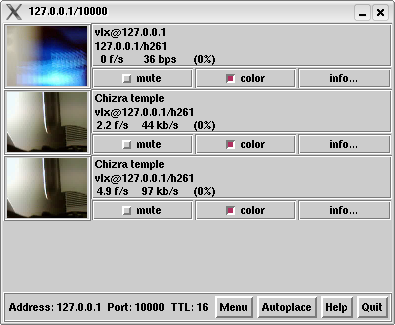
\includegraphics[width=0.3\textwidth]{images/video-app-vic-ucl}
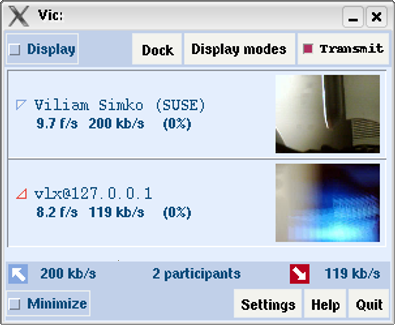
\includegraphics[width=0.3\textwidth]{images/video-app-vic-vrvs}
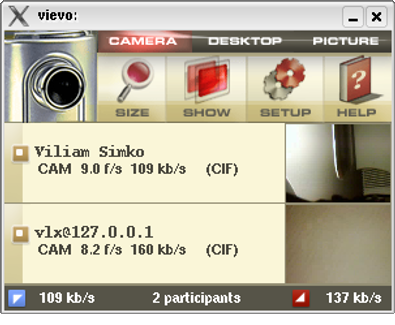
\includegraphics[width=0.3\textwidth]{images/video-app-vievo}
\caption{Aplikácie určené na prenos obrazu (vic-ucl, vic-vrvs, vievo).}
\label{fig:MBoneVideoApplications}
\end{figure}

Na obrázku \ref{fig:MBoneVideoApplications} vidíme rôzne verzie aplikácie VIC. Vľavo je originálna verzia VIC-2.8ucl1.1.3, v~strede verzia zo systému VRVS založená na upravenom OpenMash 6.1 a vpravo je značne upravená verzia z~projektu EVO, ktorá však nepatrí medzi open-source software. Tento problém sa čiastočne pokúšame riešiť reimplementáciou v~aplikácii EVIC.


\subsection{RAT}\label{kap:RAT}
Robust Audio Tool (RAT) je podobne ako aplikácia VIC určená na prenos multimediálneho obsahu v~reálnom čase pomocou RTP paketov medzi úžastníkmi multicastovej skupiny. Multimediálnym obsahom je v~prípade RATu zvuk. K~dispozícii je niekoľko zvukových kodekov, ako napr. GSM, L16 a dokonca v~niektorých verziách aj MP3. Líšia sa medzi sebou kvalitou zvuku a spotrebou prenosového pásma. Podobne ako VIC, aj RAT podporuje šifrovanie RTP obsahu a vyskytuje sa v~niekoľkých verziách, ktorých príklady vidíme na obrázku \ref{fig:MBoneAudioApplications}. Vpravo pôvodná aplikácia VAT, ktorá umožňovala prenos zvuku a obrazu súčasne, v~strede originálna verzia RAT z~balíka AG a vpravo verzia z~projektu VRVS.

V~kapitole \ref{kap:HybridRAT} je popísaná hybridná verzia aplikácie RAT, ktorá vznikla spojením zdrojových kódov z~projektu RAT-VRVS a RAT-UCL a umožňuje nahrávať zvuk pomocou sieťového loopback zariadenia (localhost). Takto opravenú verziu ponúkame záujemcom na stránkach Ciant AG node \cite{CIANT-AGnodeWiki}.

\begin{figure}
\centering
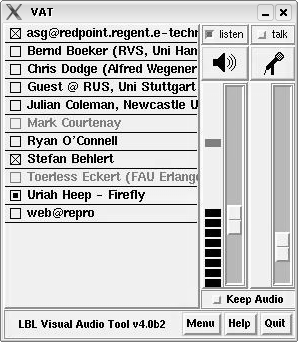
\includegraphics[width=0.3\textwidth]{images/audio-app-vat.png}
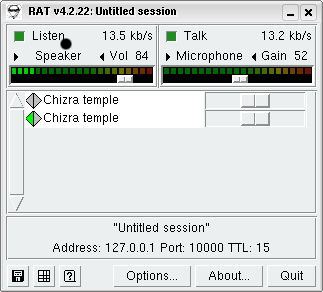
\includegraphics[width=0.3\textwidth]{images/audio-app-rat.png}
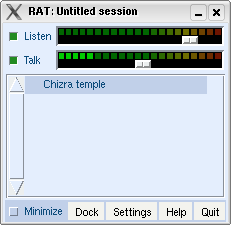
\includegraphics[width=0.3\textwidth]{images/audio-app-rat-vrvs.png}
\caption{Aplikácie určené na prenos zvuku (vat, rat, rat-vrvs).}
\label{fig:MBoneAudioApplications}
\end{figure}


%%%%%%%%%%%%%%%%%%%%%%%%%%%%%%%%%%%%%%%%%%%%%%%%%%%%%%%%%%%%%%%%%%%%%
%%%%%%%%%%%%%%%%%%%%%%%%%%%%%%%%%%%%%%%%%%%%%%%%%%%%%%%%%%%%%%%%%%%%%
\section{Shared applications}
%%%%%%%%%%%%%%%%%%%%%%%%%%%%%%%%%%%%%%%%%%%%%%%%%%%%%%%%%%%%%%%%%%%%%
%%%%%%%%%%%%%%%%%%%%%%%%%%%%%%%%%%%%%%%%%%%%%%%%%%%%%%%%%%%%%%%%%%%%%

Už v~základnej inštalácii AG sa nachádza niekoľko zdieľaných aplikácií a navyše je možné túto množinu rozšíriť pomocou jazyka Python. Architektúra zideľaných aplikácií je zázornená na obrázku \ref{fig:ArchAGSharedApp}. AG Toolkit poskytuje triedu SharedAppClient, ktorá implementuje všetky operácie potrebné pre komunikáciu pomocou zbernice Event Channel. Trieda uľahčuje doručovanie správ a synchronizáciu klientov. Komunikácia medzi klientami (Application Client) prebieha pomocou XML-RPC.

\begin{figure}
\centering
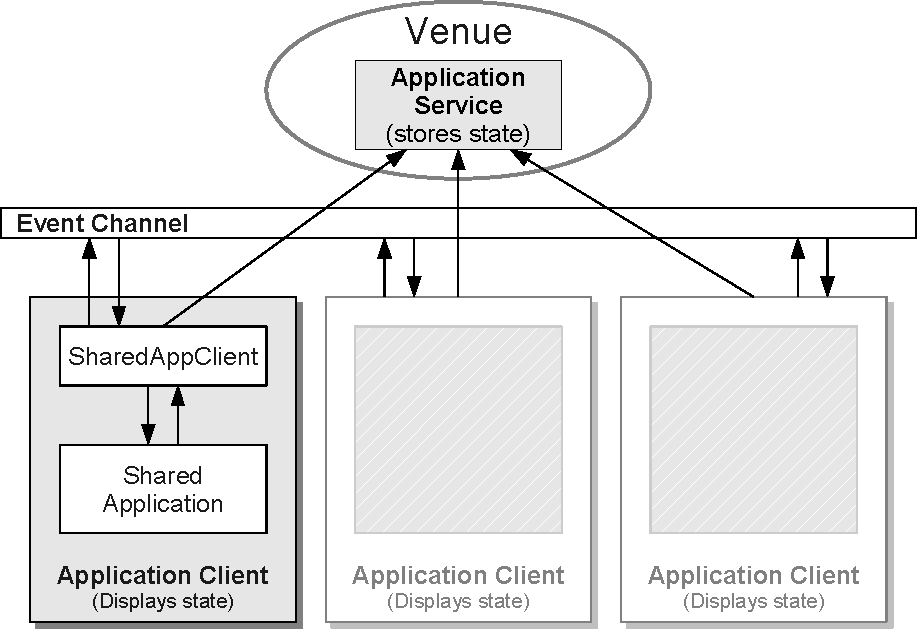
\includegraphics[width=0.8\textwidth]{images/arch-ag-sharedapp}
\caption{Architektúra zdieľaných aplikácií AccessGridu.}
\label{fig:ArchAGSharedApp}
\end{figure}

Ďalším prostriedkom pre vytvorenie zdieľaného prostredia je Virtual Network Computing (VNC) \cite{MAN-Virtual-Network-Computing}. Systém využíva Remote Frame Buffer protokol (RFB) \cite{MAN-RFB-Protocol}. Protokol prenáša informácie o~zmenách na zdieľanej obrazovke a informáciách o~stlačených klávesách a tlačítkach myši. Jeho serverová aj klientská časť je platformovo nezávislá. Protokol RFB je bezstavový a na server môže byť súčasne pripojených niekoľko užívateľov. VNC používa doručovaciu metódu unicast, takže môže vzniknúť problém pri veľkom množstve účastníkov. Projekt VNCast \cite{Vislab-VNCast} by mal prenášať VNC pomocou multicastových služieb tak, že zakóduje VNC obraz pomocou Motion JPEG (kapitola \ref{kap:MJPEG}) do RTP paketov. Zatiaľ je však iba v~štádiu vývoja.

Pomocou schémy na obrázku \ref{fig:PresentationFileFormats} chceme poukázať na možnosť využitia VNC ako integračného nástroja formátov, pre ktoré neexistuje špeciálna zdieľaná aplikácia. Uvažujeme o~možnosti nahrávania obrazu z~VNC vo forme RTP paketov alebo pomocou vncproxy/vncrec/transcode.

\begin{verbatim}
# Príklad prevodu VNC obrazu do formátu XviD
vncrec -record file.vnc :0
transcode -x vnc -y xvid -i file.vnc -o file.avi -z -k
\end{verbatim}

Komunikáciu protokolom XML-RPC nie je možné nahrávať tak jednoducho ako RTP alebo RFB pakety. Pre účely nahrávania by bolo najvýhodnejšie vysielať vedľa bežného obrazu aj snímky pracovnej plochy.

\begin{figure}
\centering
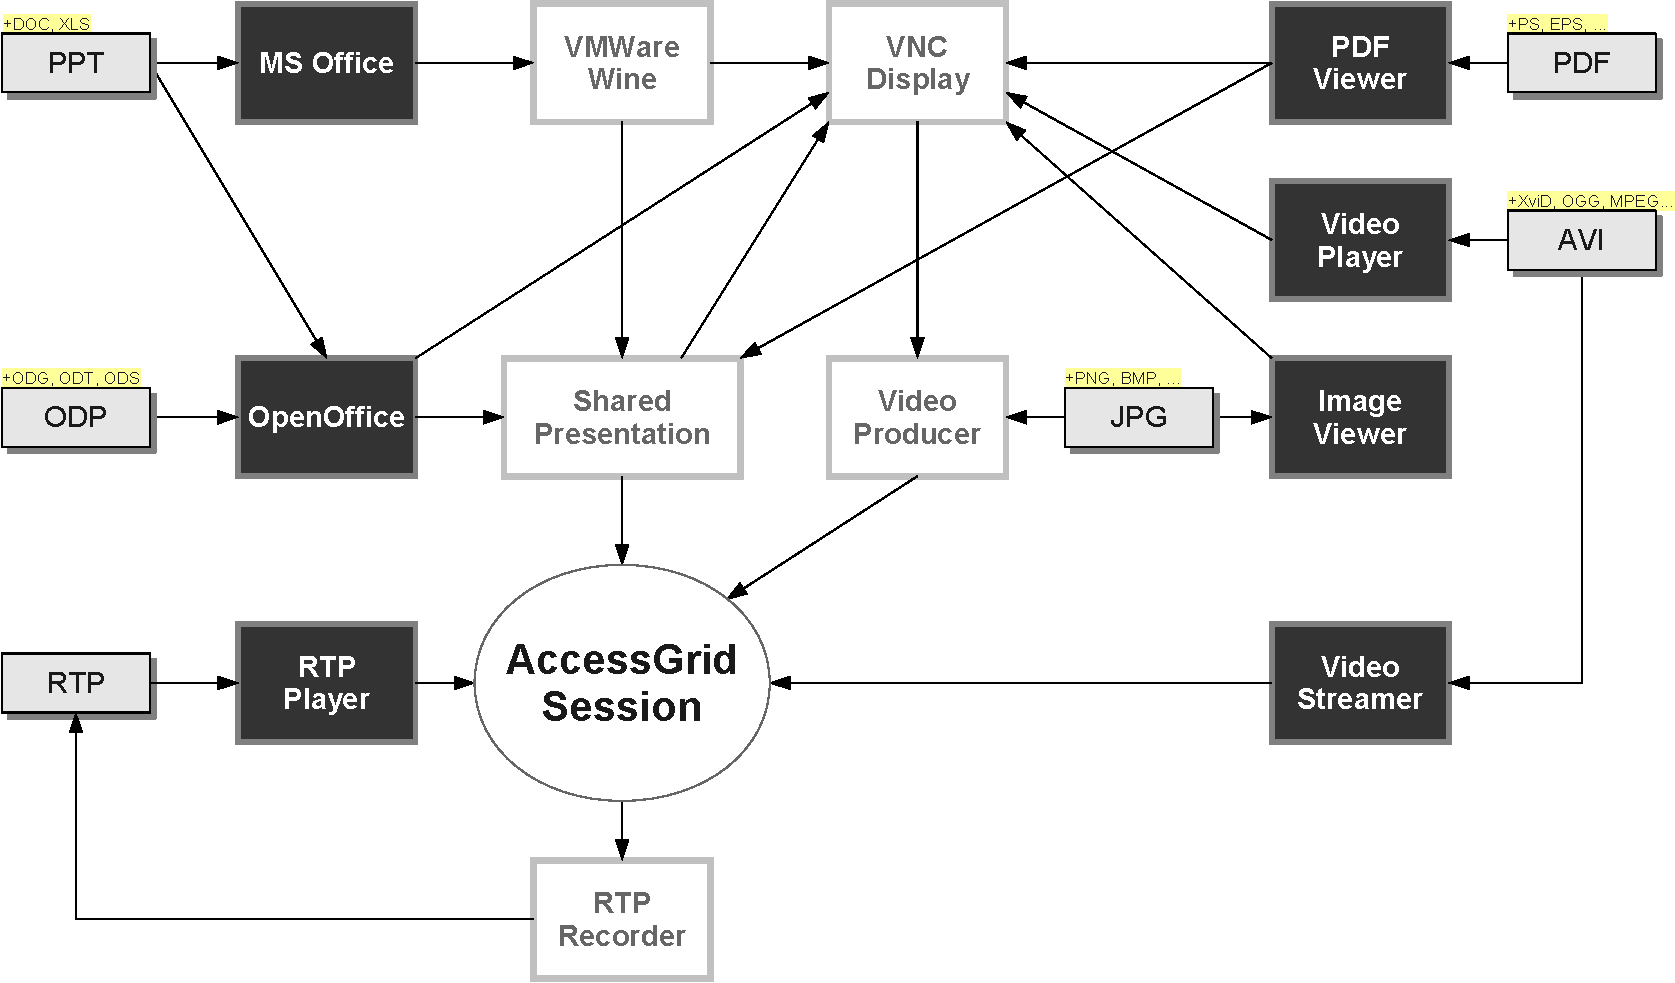
\includegraphics[width=1\textwidth]{images/vc-input-formats}
\caption{Využitie rôznych formátov v~prezentácii.}
\label{fig:PresentationFileFormats}
\end{figure}

Len pre úplnosť uvádzame, že existuje ešte robustnejší protokol pôvodom z~Microsoft Terminal Services s~názvom \textbf{RDP ITU T.128}, ktorý prenáša aj zvuk, súbory a zdieľané disky. V~tejto práci však budeme používať jednoduchší systém VNC.


\subsection{Shared presentations}
Linuxová verzia AG 2.4 obsahuje nástroje SharedBrowser, SharedPresentation a SharedPDF. \textbf{SharedPresentation} používa OpenOffcie pre zobrazovanie prezentácií vo formáte PPT (MS PowerPoint), ODP (Open Document Presentation) a SXI (Staršia verzia OpenOffice/StarOffice). \textbf{SharedPDF} umožňuje zdieľať prezentácie uložené vo~formáte PDF a pod Linuxom využíva aplikáciu xpdf. \textbf{SharedBrowser} využíva internetový prehliadač Mozilla.

Užívateľ iste narazí na niekoľko nepríjemných chýb (alebo vlastností?) týchto aplikácií. V~prípade SharedPDF sa zobrazujú vždy dve rovnaké okná s~PDF dokumentom, pričom by stačilo len jedno. Využitie by iste našla aj podpora pre prehliadač KPDF. V~prípade SharedBrowser musí byť ručne doinštalovaný modul pre Python, ktorý vytvorí rozhranie pre prehliadač Mozilla, inak aplikácia nefunguje. Navyše chýba podpora pre prehliadače Konqueror a Opera. SharedPresentation zas neumožňuje ovládanie fullscreen prezentácie a chýba filter pre súbory s~príponou ODP. Opravenú verziu ponúkame záujemcom na stránkach projektu Ciant AG node \cite{CIANT-AGnodeWiki}.

\subsection{Shared desktop}
AccessGrid tiež obsahuje dva VNC nástroje -- starší VenueVNC a jeho nástupcu SharedDektop \cite{AG-SharedDesktop}. Zdieľanú pracovnú plochu je možné využiť nielen pri prezentáciách ale aj ako nástroj pri riešení technických problémov.

Zaujímavý projekt sľubujú stránky Vislabu, ktoré popisujú aplikáciu SharedDesktop \cite{Vislab-SharedDesktop}. Zmenou oproti klasickému VNC je prenos zvuku, 3D akcelerácia a zobrazovanie kurzorov myši všetkých pripojených klientov. Vývoj tejto aplikácie však postupuje veľmi pomaly a zatiaľ neexistuje žiadna použiteľná verzia.

\subsection{Shared media player}
Aplikácia Shared Media Player bola zatiaľ doménou výlučne operačného systému Windows \cite{AG-SharedMoviePlayer}. Rozhodli sme sa preto vytvoriť zdieľanú aplikáciu podobného typu aj pre systém Linux. Riešenie sa opiera o~schopnosti prehrávača MPlayer, ktorý je dostupný pre široké spektrum unixových operačných systémov a dokonca aj pre systém Windows. Pri tvorbe sme vychádzali z~aplikácie SharedPDF, ktorá umožňuje zdieľanú prezentáciu PDF dokumentov. Rozhranie k~xpdf sme nahradili rozhraním k~aplikácii MPlayer.

Inštalačný balík poskytujeme na wiki-stránkach projektu Ciant AG node \cite{CIANT-SharedMPlayer}. Inštalácia vyžaduje spustenie príkazu:
\begin{verbatim}
agpm.py -z SharedMPlayer.zip
\end{verbatim}

\subsection{Further shared applications}
Pre úplnosť by sme ešte radi spomenuli aplikáciu \textbf{SharedRasmol} \cite{AG-SharedRasmol}, ktorá umožňuje 3D vizualizáciu molekúl, \textbf{Shared Question Tool} \cite{AG-SharedQuestionTool} pre zdieľanú tvorbu otázok a odpovedí a \textbf{AGBasicImage}, ktorá umožňuje zdieľané prezeranie obrázkov a úpravu ich metadát.
Ďalej \textbf{Media Lecture Board}, ktorá umožňuje zdieľanú tvorbu dokumentov. V~praxi sa však ukázala ako veľmi nestabilná.

%%%%%%%%%%%%%%%%%%%%%%%%%%%%%%%%%%%%%%%%%%%%%%%%%%%%%%%%%%%%%%%%%%%%%
%%%%%%%%%%%%%%%%%%%%%%%%%%%%%%%%%%%%%%%%%%%%%%%%%%%%%%%%%%%%%%%%%%%%%
\section{G-Ware configuration tool}
%%%%%%%%%%%%%%%%%%%%%%%%%%%%%%%%%%%%%%%%%%%%%%%%%%%%%%%%%%%%%%%%%%%%%
%%%%%%%%%%%%%%%%%%%%%%%%%%%%%%%%%%%%%%%%%%%%%%%%%%%%%%%%%%%%%%%%%%%%%

Zariadenia na potlačenie spätnej väzby od firmy ClearOne (predtým Gentner) sa konfigurujú pomocou jednotného nástroja G-Ware.
AG uzol v~organizácii CIANT využíva verziu AP-800. Ešte donedávna bola situácia komplikovaná tým, že software existuje iba vo verzii pre operačný systém Windows. Aplikácia sa síce používa iba pri výrazných zásahoch do parametrov miestnosti, ale bolo nutné vlastniť aspoň jednu licenciu na inak nevyužívaný operačný systém. Najnovšie verzie Wine a CrossoverOffice však už bezproblémov dokážu tento nástroj emulovať v prostredí Linuxu (obrázok \ref{fig:GWareInWine}). Tým skončila posledná závislosť na OS Windows. Inštalačný balík G-Ware s~veľkosťou cca 20MiB je možné získať na stránkach výrobcu ClearOne \cite{ClearOne-ResourceLibrary} spolu so~všetkými potrebnými manuálmi.

Detailný popis inštalácie pre staršie verzie Wine poskytujú stránky Vislabu \cite{Vislab-GWare}, autori popisujú kompiláciu zo zdrojových kódov vrátane potrebného patch súboru.

\begin{figure}
\centering
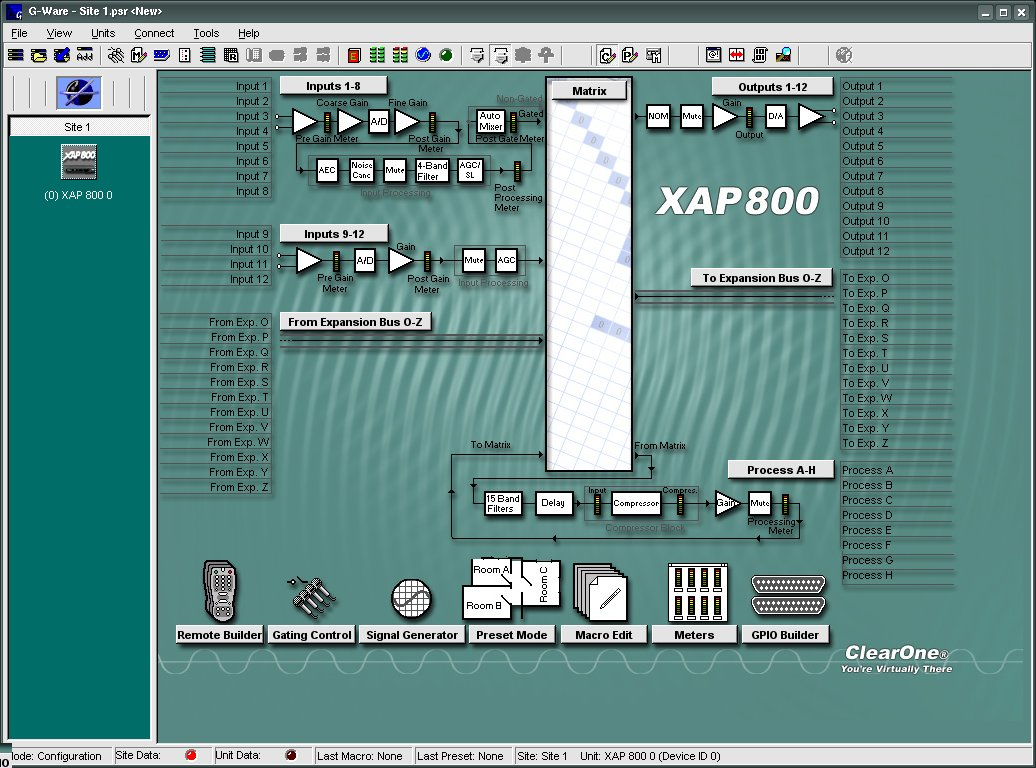
\includegraphics[width=0.9\textwidth]{images/gware}
\caption{G-Ware emulovaný pomocou Wine.}
\label{fig:GWareInWine}
\end{figure}

%%%%%%%%%%%%%%%%%%%%%%%%%%%%%%%%%%%%%%%%%%%%%%%%%%%%%%%%%%%%%%%%%%%%%
%%%%%%%%%%%%%%%%%%%%%%%%%%%%%%%%%%%%%%%%%%%%%%%%%%%%%%%%%%%%%%%%%%%%%
\section{Bridging the multicast}
%%%%%%%%%%%%%%%%%%%%%%%%%%%%%%%%%%%%%%%%%%%%%%%%%%%%%%%%%%%%%%%%%%%%%
%%%%%%%%%%%%%%%%%%%%%%%%%%%%%%%%%%%%%%%%%%%%%%%%%%%%%%%%%%%%%%%%%%%%%

Architektúra AccessGridu je do veľkej miery závislá na multicastovom pripojení. Jeho správne fungovanie sa overuje pomocou nástroja Multicast Beacon. Môže však nastať situácia, kedy niektorý z~uzlov dočasne alebo permanentne nepodporuje multicast. Problémy spojené s~dostupnosťou muticastu je možné rozdeliť na 3 skupiny:

\begin{enumerate}
\item Sieť bez podpory multicastu.
\item Vznik izolovaných multicastových oblastí.
\item Problémy spojené s~prechodom cez NAT a firewall.
\end{enumerate}

V~historii AccessGridu sa objavilo niekoľko pokusov o~prekonanie týchto problémov. Vznikli tak projekty RCBridge, QuickBridge, AGConnector a komerčný InSORS Enterprise Manager.

\paragraph*{RCBridge:}
Je nástroj napísaný v~jazyku Java s~webovým rozhraním, ktorý forwarduje pakety medzi multicastovou a unicastovou sieťou. Nástroj však nie je integrovaný s~architektúrou AccessGridu.

\paragraph*{QuickBridge:}
Je jednoduchý UDP forwarder napísaný v~jazyku C, ktorý je dodávaný ako súčasť inštalačného balíka AccessGridu 2.4. Nevýhodou je neúspech pri prekonávaní NAT.

\paragraph*{AGConnector:}
Riešenie založené na myšlienke tunelovania multicastových paketov pomocou jedného UDP spojenia. Obsahuje dva hlavné komponenty -- UMTP Agent a UMTP Server. Táto aplikácia existuje len pre AccessGrid 3.0.

\paragraph*{InSORS Enterprise Manager:}
Komerčné riešenie, ktoré okrem multicastového mostu ponúka navyše H.323 bridge a IG Pix Presentation Server pre nahrávanie zdieľaných prezentácií.


\subsection{QuickBridge}

Funkcia komponentu QuickBridge je znázornená na obrázku \ref{fig:QuickBridge}. Aplikácia preposiela pakety medzi multicastovou sieťou a unicastovými uzlami použité UDP porty je možné ľubovolne nastavovať. Detailná dokumentácia, popis inštalácie a zdrojové kódy sa nachádzajú na stránkach projektu AccessGrid \cite{AG-BridgingGuide}.

Pre zjednodušenie si predstavme nasledujúcu situáciu: Všetky uzly odosielajú a prijímajú UDP pakety na multicastovej adrese 224.0.0.1 na porte 10000. Jedným z~uzlov je aj QuickBridge, ktorý navyše akceptuje unicastové spojenia vo forme UDP paketov na porte 20000. QuickBridge si vedie zoznam aktívnych uzlov, ktoré mu poslali UDP pakety na tento port. Každý UDP paket z~unicastovej siete preposiela do multicastovej siete a naopak. Pokiaľ unicastový uzol po istú dobu neodpovedá, QuickBridge ho vyškrtne zo zoznamu a už mu nepreposiela nové pakety. Takúto jednoduchú situáciu môžeme namodelovať príkazom:
\begin{verbatim}
QuickBridge -g 224.0.0.1 -m 10000 -u 20000
\end{verbatim}

V~prostredí AccessGridu sa QuickBridge konfiguruje vždy pre nejaký VenueServer a to pomocou konfiguračného súboru \textbf{BridgeServer.cfg}. Ako príklad konfigurácie môžeme uviesť existujúce nastavenie pre uzol v~organizácii CIANT, ktorý sme popisovali v~kapitole \ref{kap:CIANT-AG-Bridge}. Bridge je potom možné spustiť príkazom:
\begin{verbatim}
BridgeServer.py -c ./BridgeServer.cfg
\end{verbatim}

\begin{verbatim}
# BridgeServer.cfg
[BridgeServer]
name = CiantMagicUnicastBridge
location = Prague
qbexec = /usr/bin/QuickBridge
BRIDGESERVER = CiantMagicUnicastBridge
\end{verbatim}

\begin{verbatim}
# Use this port range for the bridge server as a whole
portMin = 20000
portMax = 20005
\end{verbatim}

\begin{verbatim}
# Name of Lobby that you wish to provide a bridge to
[https://195.113.187.114:8000/Venues/default]
type = Venue
\end{verbatim}

\begin{figure}
\centering
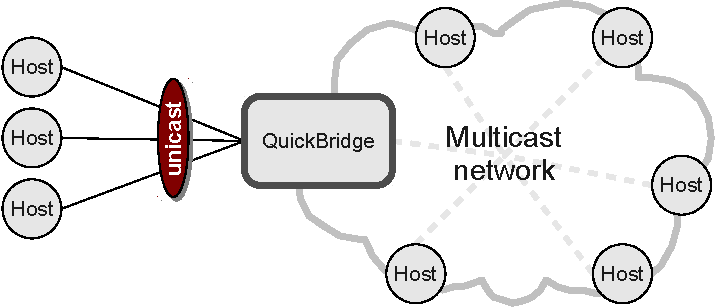
\includegraphics[width=0.7\textwidth]{images/arch-quickbridge}
\caption{Premostenie multicastu pomocou QuickBridge.}
\label{fig:QuickBridge}
\end{figure}

Problém použitia QuickBridge v~prostredí s~NAT spočíva vo vlastnosti  protokolov RTP/RTCP. Pre jedno dátové spojenie sa používajú vždy dva UDP porty -- $2k$ pre RTP a $2k+1$ pre RTCP. Cez NAT tak prejde RTCP informácia ale opačným smerom už RTP neprejde.

\subsection{AGConnector}
Tento software nahradzuje QuickBridge v~novej verzii AccessGridu (verzia 3.0). Rieši problém prenosu multicastových paketov medzi multicastovými ostrovmi, špeciálne prípad siete za firewallom a NATom. AGConnector využíva protokol UMTP \ref{kap:UMTP}, pomocou ktorého tuneluje multicastové UDP pakety medzi multicastovými ostrovmi (obrázok \ref{fig:AGConnector}). Prenos zabezpečuje jediný UDP port 8010 UDP, ktorý nesmie byť blokovaný firewallom. Inštalácia prebieha príkazom:
\begin{verbatim}
agpm.py –z AG_Connector.zip
\end{verbatim}

\begin{figure}
\centering
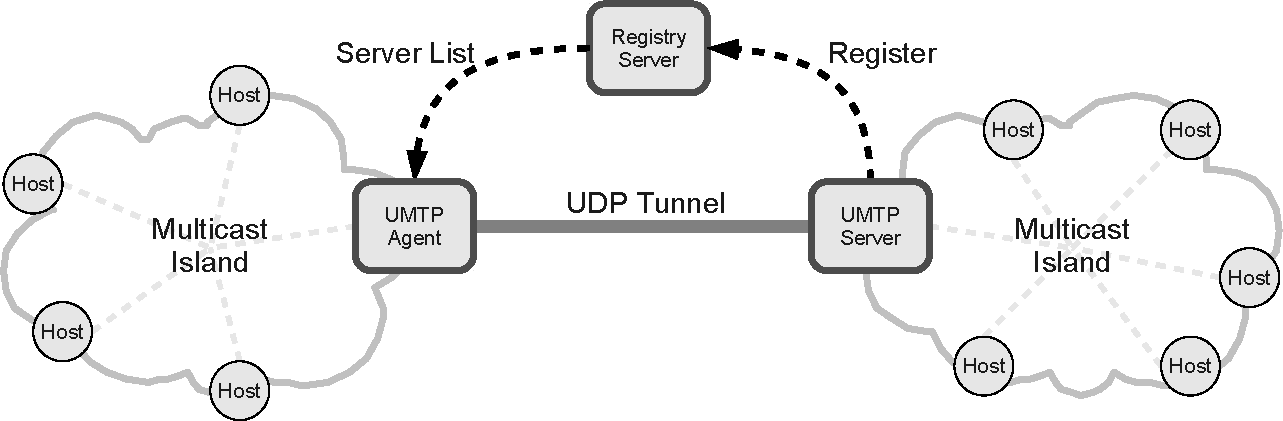
\includegraphics[width=1\textwidth]{images/arch-agconnector}
\caption{Premostenie multicastu pomocou AGConnector. (zdroj \protect\cite{AG-Connector})}
\label{fig:AGConnector}
\end{figure}

%%%%%%%%%%%%%%%%%%%%%%%%%%%%%%%%%%%%%%%%%%%%%%%%%%%%%%%%%%%%%%%%%%%%%
%%%%%%%%%%%%%%%%%%%%%%%%%%%%%%%%%%%%%%%%%%%%%%%%%%%%%%%%%%%%%%%%%%%%%
\section{Results and suggestions}
%%%%%%%%%%%%%%%%%%%%%%%%%%%%%%%%%%%%%%%%%%%%%%%%%%%%%%%%%%%%%%%%%%%%%
%%%%%%%%%%%%%%%%%%%%%%%%%%%%%%%%%%%%%%%%%%%%%%%%%%%%%%%%%%%%%%%%%%%%%
Všetky komponenty potrebné pre chod plnohodnotného AccessGridového uzla je možné prevádzkovať v~operačnom systéme Linux. Problémovými aplikáciami boli G-Ware a SharedMediaPlayer. V~rámci tejto práce sme vytvorili zdieľanú aplikáciu SharedMPlayer, ktorá poskytuje podobné funkcie ako SharedMediaPlayer pre Windows. Navyše ťažíme z~obrovského množstva kodekov, ktoré podporuje MPlayer. Ostatné zdieľané aplikácie, ktoré sme popisovali, existujú pre obe platformy. G-Ware je možné emulovať v~prostredí Wine.

Stav videokonferenčného uzla je potrebné preventívne testovať. Pre tento účel usporiadava komunita AG pravidelné stretnutia zameraná na odhaľovanie a odstraňovanie problémov za pomoci skúsených užívateľov AG. Užitočné informácie o~odstraňovaní problémov so zvukom, obrazom, sieťovým pripojením a zdieľanými aplikáciami sa nachádzajú priamo na stránkach AG \cite{AG-QualityAssurancePreparation}.

\proofed
